%---------- Inleiding ---------------------------------------------------------

\section{Introductie}%
\label{sec:introductie}

Kubernetes is een snel opkomende en krachtige opensourcesoftware voor het automatiseren en beheren van containers. Deze containers kunnen Docker of een andere technologie zijn. Om deze containers te laten communiceren en samenwerken, worden deze toegepast binnen een Kubernetes cluster. 

Een Kubernetes cluster, ook wel een k8s genoemd, is een groep van noden. Deze groep noden bestaan uit minstens één master node en een aantal worker nodes. Binnen deze worker nodes zijn er pods waarin containers draaien. \textit{Figuur 1} brengt hier meer duidelijkheid over. Deze containers bevatten applicaties zoals een SQL database of een website die draait met nginx. In de literatuurstudie wordt dit uitgebreid besproken.

De scope van dit onderzoek omvat alles wat te maken heeft met Docker containers te beveiligen binnen een Kubernetes cluster. De configuratie van de applicaties binnen deze containers zijn niet van toepassing in deze paper. In dit onderzoek worden tools zoals kubehunter en kube-bench besproken voor het analyseren en het uitvoeren van beveiligings checks. 


Hoe scherm je het best een container af van bedreigingen of aanvallen? Elke laag binnen een node, zoals een pod en een container moet geïsoleerd en beschermd zijn tegen aanvallen en bedreigingen.

Hoe kan een container direct beveiligd zijn bij een deployment?

Tot hoe ver kan men gaan bij het scannen en analyseren van Docker images in een pipeline?

\begin{flushleft}
    \begin{figure}[h]
        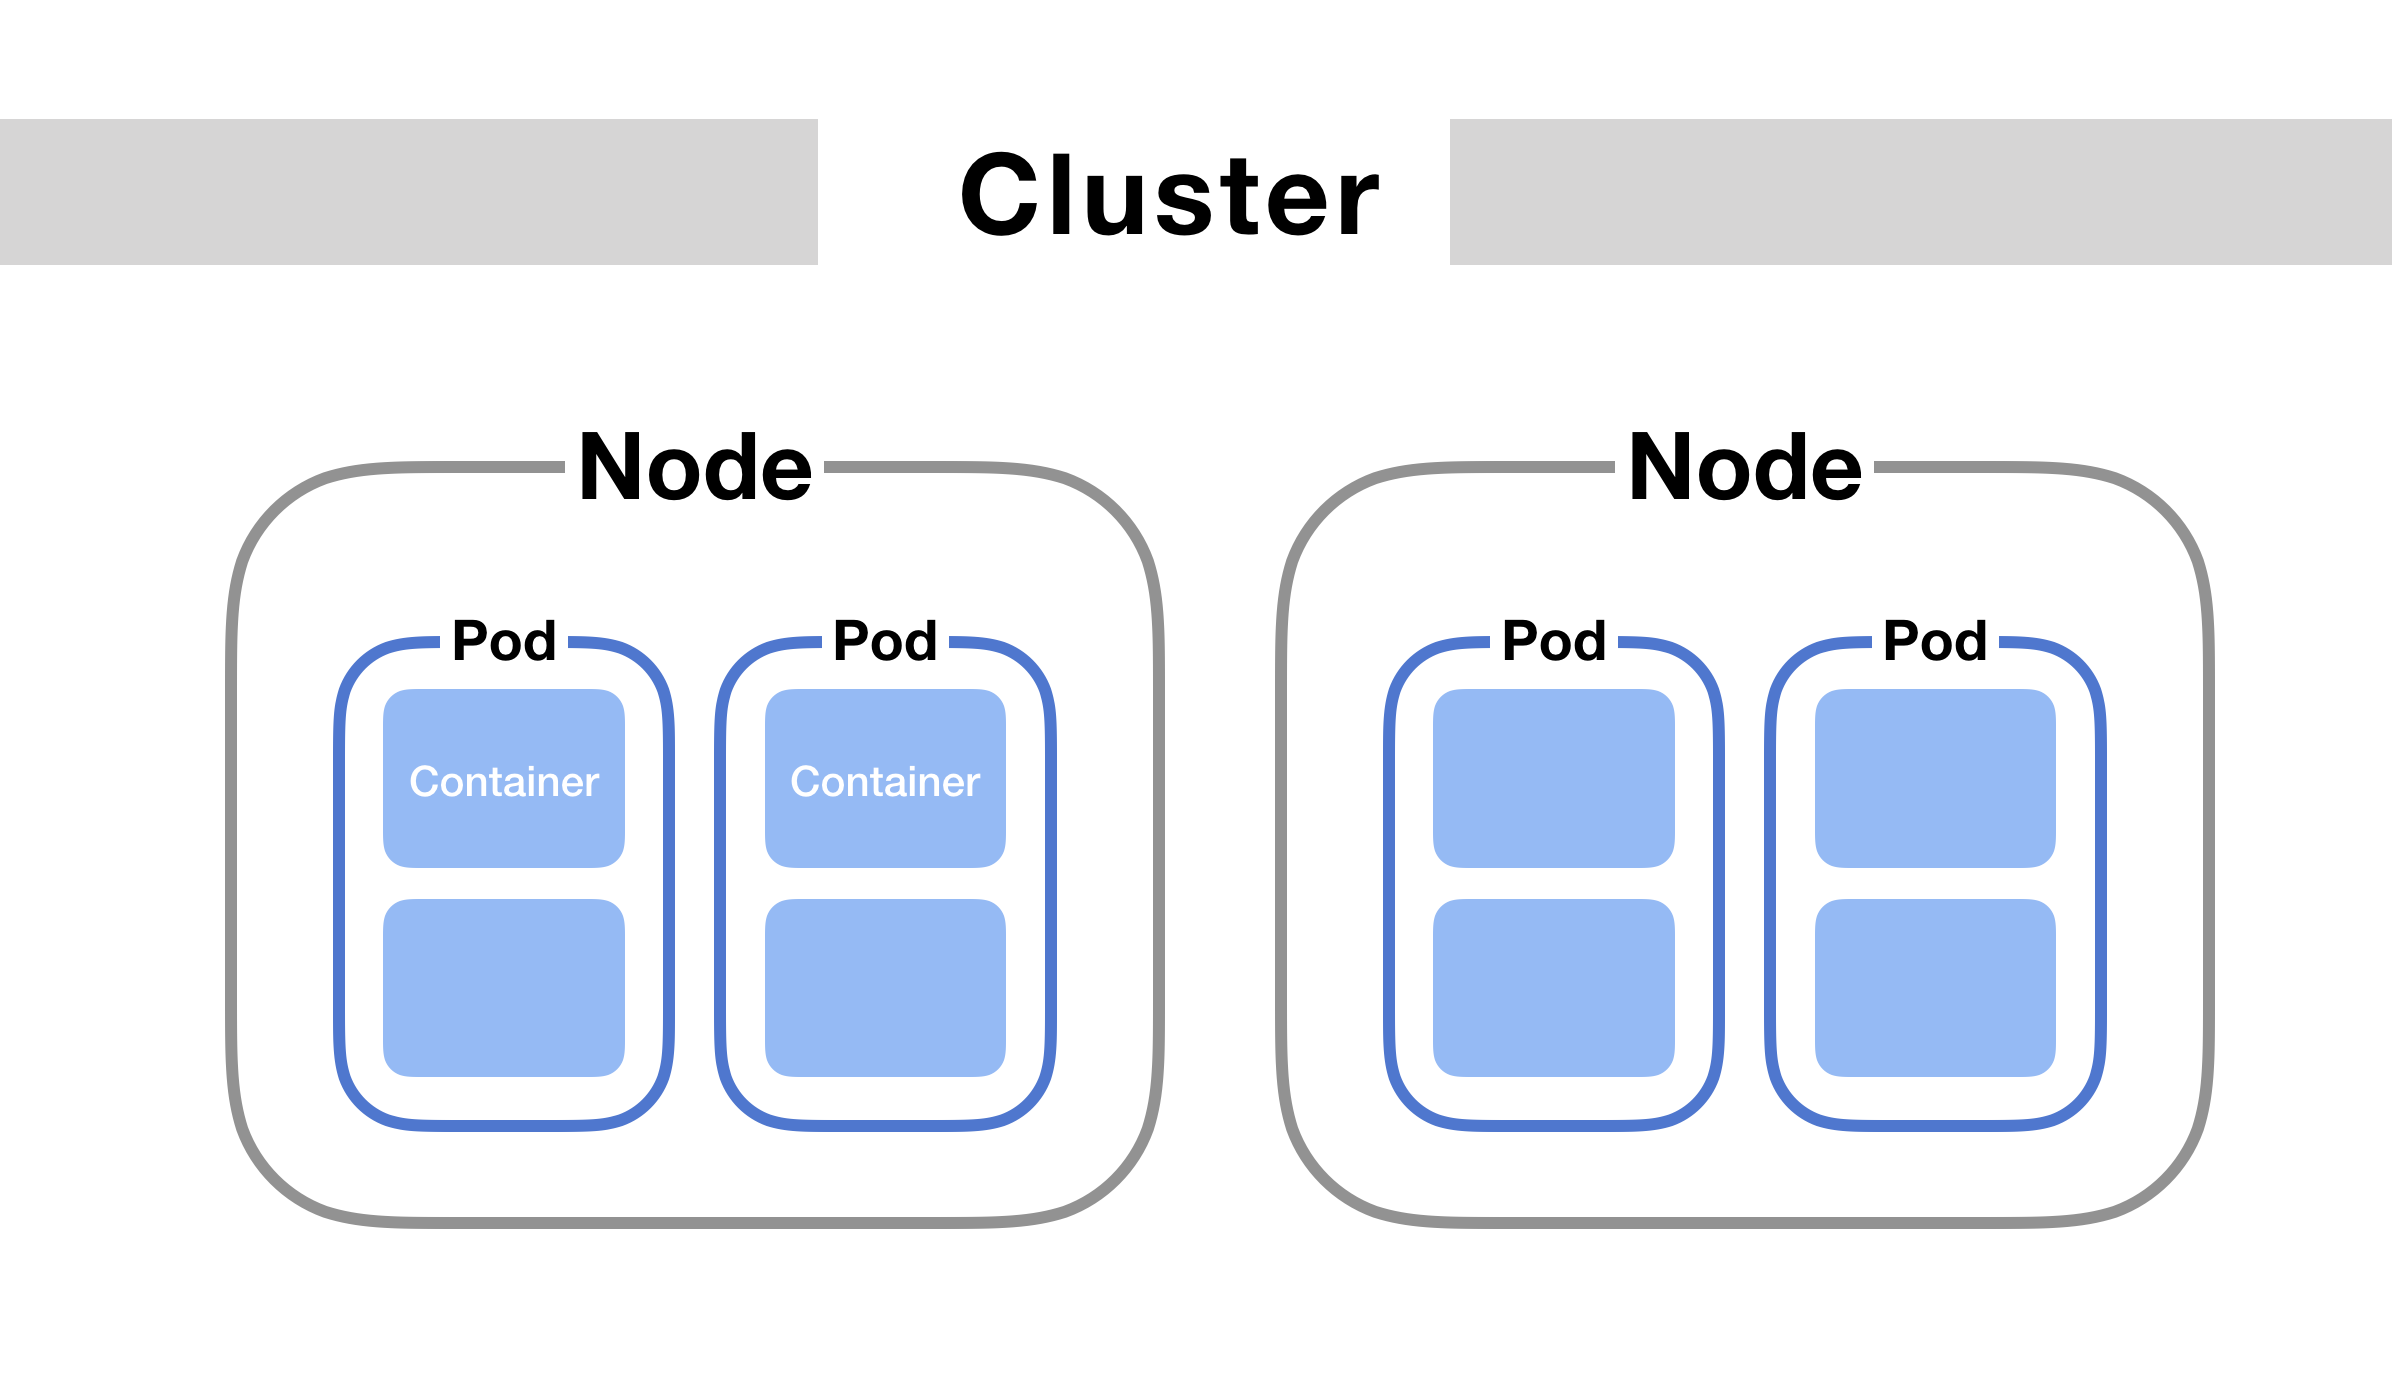
\includegraphics[width=.49\textwidth]{img/node-overview.png}
        \caption{\label{fig:Kubernetes 4c}Kubernetes cluster with nodes \autocite{kubernetes-MP}}
    \end{figure} 
\end{flushleft}

Securex, een sociaal zekerings bedrijf gevestigd in gent, maakt gebruik van een Kubernetes omgeving met Docker containers om hun applicaties te laten draaien. Een belangrijk aspect van het gebruik van deze containers is de beveiliging ervan. Zonder effectieve beveiligingsmaatregelen en isolatie van de containers en de Kubernetes omgeving kunnen deze containers blootgesteld worden aan beveiligingsrisico's. Als deze containers gevoelige informatie bevatten kan dit erge gevolgen hebben voor Securex.

Securex verwacht dat de beveiliging van een Docker container in een Kubernetes omgeving zo volledig mogelijk in kaart wordt gebracht. Dit houdt in dat de verschillende tools, bedreigingen en oplossingen uitvoerig onderzocht worden. Het resultaat van dit onderzoek zal Securex in staat stellen om hun containers beter te isoleren en beschermen tegen bedreigingen en beveiligingsrisico's.


%---------- Stand van zaken ---------------------------------------------------

\section{Literatuurstudie}%
\label{sec:Literatuurstudie}

\autocite{Allclair2018} Om de beveiliging van een container te optimaliseren moet er laag per laag geïsoleerd worden. De eerste laag is de infrastructuur laag. Dit is het netwerk gedeelte buiten Kubernetes en valt buiten de scope van dit onderzoek. 


Na de infrastructuur laag bevindt zich de Kubernetes cluster. De cluster is het geheel van de Kubernetes omgeving. Hierin bevindt zich de control plane en een aantal worker nodes. 
De control plane bestaat uit master nodes die de worker nodes beheren. 
\autocite{kubernetesDocs-2022} Pods, Namespaces, ConfigMaps en Events kunnen via de API server in de master node aangepast worden via een user interface of kubectl, een command-line tool van Kubernetes. De eindgebruiker heeft directe toegang met de API server om deze worker nodes te beheren. Iemand met root toegang tot deze command-line kan dus de gehele cluster beheren. \autocite{sayfan-2020} Een ander cruciaal component in de control plane is etcd. Dit is een data stored bestand die de staat van de cluster bijhoud. Naast etcd en de API server is er ook de Scheduler \autocite{Huss2019}, die zorgt ervoor dat er bij deployment van pods rekening gehouden word met de middelen van de node. Als er bijvoorbeeld 6 pods gecreëerd moeten worden dan gaat de Scheduler dit verdelen over de beschikbare nodes. Als zo een node uitvalt dan gaat hij automatisch de verloren pods verdelen over de andere nodes.


De volgende laag is de node laag. Een node bestaat uit één of meerdere pods die elk een container bevatten. In elke node is er een kubelet. Kubelets dienen voor de communicatie tussen de API server en een node. \autocite{Rice2018} De standaard communicatie tussen een API server en een kubelet is via http en dus onveilig omdat er geen end-to-end encryptie is. Dit maakt het mogelijk voor man-in-the-middle aanvallen.
\autocite{kubernetespods-2022} Een pod bevat niet alleen containers, maar ook middelen zoals volumes en ook een eigen ip adres. Het is aangeraden om alleen één container per pod te draaien tenzij de containers aan elkaar vast hangen en elkaar nodig hebben om te functioneren. Als er zich in een pod kwetsbaarheden bevinden en er toegang word gegeven aan de volumes kan dit de data in deze volumes in gevaar brengen.


Ten slotte is de laatste laag de container. Dit hoort niet specifiek tot Kubernetes, maar behoort wel in de scope van dit onderzoek. Volgens onderzoek van \textcite{Rice2018} kunnen de images die gebuild worden, ook worden gescand op kwetsbaarheden. Dit kan geintegreerd worden in een CI/CD pipeline waarbij ze voor het deployen van de container eerst gaan checken op bekende kwetsbaarheden. 


%---------- Methodologie ------------------------------------------------------
\section{Methodologie}%
\label{sec:methodologie}

De eerste fase van het onderzoek is het opzetten van een test omgeving van Kubernetes met minikube.\autocite{kubernetesMinicube-2022} Minikube is een implementatie van Kubernetes dat een VM creëert op je hostsysteem en een cluster bevat met één node. De CLI van minikube heeft de basisch commando's voor onder andere het stoppen, starten, deleten van een cluster. 

In het tweede luik van het onderzoek wordt er laag per laag onderzocht welke kwetsbaarheden voorkomen bij deployen van een basisch container binnen een Kubernetes cluster zonder beveiligingsmaatregelen. Popeye, kube-bench en kube-hunter zijn enkele tools om deze kwetsbaarheden te onderzoeken.

In de derde fase van het onderzoek worden de nodige beveiligingsprincipes toegepast op de verschillende lagen binnen Kubernetes. Startend van de cluster laag, eindigend met de containers. Deze beveiligingsprincipes zijn gebaseerd op de security manual van securex. Om zo rekening te houden met gebruikersrechten en nodige poorten of services die moeten open staan.

Tot slot wordt er gekeken hoe deze beveiligingsprincipes kunnen toegepast worden bij het ontplooien van een k8s met een container. Er wordt onderzocht hoe direct alle lagen geïsoleerd kunnen zijn, zonder de User Interface te gebruiken.

%---------- Verwachte resultaten ----------------------------------------------
\section{Verwacht resultaat, conclusie}%
\label{sec:verwachte_resultaten}

Uit dit onderzoek wordt er verwacht dat Securex in staat is om veilig containers op te zetten in de productieomgeving. Maar zo een container kan niet maanden of weken aan een stuk goed beveiligd zijn. Bij elke update of patch van Kubernetes, Docker of een andere gebruikte tool of programma binnen de omgeving, kunnen er nieuwe kwetsbaarheden opduiken. Daarom is het belangrijk dat deze updates strikt moeten worden opgevolgd om een zo veilig mogelijke structuur aan te houden.

